%%%%%%%%%%%%%%%%%%%%%%%%%%%%%%%%%%%%%%%%%%%%%%%%%%%%
%    Canadian AI Latex Template    %
%%%%%%%%%%%%%%%%%%%%%%%%%%%%%%%%%%%%%%%%%%%%%%%%%%%%
\documentclass[10pt]{cai}

\begin{document}
% Editorial staff will replace the following values:
% 1. Conference Year
% 2. Issue number
% 3. Article DOI
\def\conferenceyear{2025}
\volumeheader{38}{0}%{00.000}
\begin{center}

\title{Development of a Reinforcement Learning Enabled Cattle Tracker Prototype}
\maketitle

\thispagestyle{empty}

% Add Authors and Affiliations in the camera ready
% for the double blind review, please leave this section as is 
\begin{tabular}{cc}
First Author\upstairs{\affilone,*}, Second Author\upstairs{\affilone}, Third Author\upstairs{\affilthree}
\\[0.25ex]
{\small \upstairs{\affilone} Affiliation One} \\
{\small \upstairs{\affiltwo} Affiliation Two} \\
{\small \upstairs{\affilthree} Affiliation Three} \\
\end{tabular}
  
% Replace with corresponding author email address
\emails{
  \upstairs{*}corresponding\_author@example.ca 
}
\vspace*{0.2in}
\end{center}

\begin{abstract}
This is just a sample \LaTeX template. As usual, most of the customization for the proceedings is done in the \texttt{cai.cls} file. 
\end{abstract}

% add your keywords
\begin{keywords}{Keywords:}
Internet of Things (IoT), reinforcement learning.
\end{keywords}
\copyrightnotice

\section{Introduction}

There is an estimated 1.5 million beef cows in Alberta with a portion of those being free-range cattle who are allowed to graze on large pastures for extended periods of time.
Many farmers and researchers are interested in tracking movement of these cattle to asess the health of the herd, and to monitor the location of the cattle.
These trackers take the form of collars, or ear tags and are equipped with sensors, batteries, and communication modules.
The installation of the trackers is often a time consuming process so a tracker is expected to operate for extended periods of time (months) without human intervention.
Given the size of the devices and the environment that they are expected to operate in, there is a limited amount of power budget available to the device and it beocmes a balancing act to ensure contiunuous operation, transmission and data collection.
Reasearchers would like a device that transmits information at high rates as higher fidelity information allows them to make better conclusions about the state of the herd.
Sensors data that researchers are interested in includes GPS coordinates, accelerometer data snapshots, and temperature data.

The paradigm of Internet of Things (IoT) devices has emerged over the last two decade as a way to deploy compute and intelligence throughout the environment.
% The number of IoT devices is expected to grow to 75 billion by 2025 \cite{gubbiInternetThingsIoT2013}.
The devices are often small, low power, and have limited communication capabilities, but provide insights into the environment that they are deployed in.
The cattle trackers are an example of an IoT device that is deployed in the environment to provide insights into the health and location of the herd.
IoT devices combine sensors, communication modules, storage, and compute to provide insights into the environment that they are deployed in.
IoT devices come as networks or individual devices and in the case of a cattle tracker, ideally a tracker would be self-sufficient as a stand-alone item.
With the spread of the internet and Starlink-like services, it is possible to have a tracker that is connected to the internet and can send data to the cloud, which enables the farmer to monitor the herd from anywhere in the world.
Again we have the challenge of limited power budget and the need to transmit data at high rates.
The power budget can be extended with the use of solar power. 
Solar power is susceptible to weather conditions and the amount of sunlight that is available to the device, which in the case of cattle trackers also depends on the location/orientation of the cattle.

Reinforcement learning is a branch of machine learning that is allows an agent to learn optimum actions to take in an environment to maximize a reward.
The agent learns these actions by interacting with the environment and receiving feedback on the actions that it takes.
Reinforcement learning has been used in a variety of applications such as playing games, optimizing energy consumption, and optimizing the operation of IoT devices.
Machine learning deployed on IoT devices is somtimes referred to as Artificial intelligence of Things (AIoT)\cite{yamsaniIoTBasedLivestockMonitoring2024}, which includes a broad range of applications.
The TinyML paradigm is a subset of AIoT and focuses on machine learning on devices with highly constrained resources, which often limits it to inference only\cite{rayReviewTinyMLStateoftheart2022}.
On one hand the addition of intelligence to the device allows it to make better decisions, but on the other hand the addition of intelligence to the device increases the power consumption of the device.
Q-learning is a reinforcement learning algorithm that is used to optimize the actions that an agent takes in an environment and has been used in a variety of applications such as optimizing the operation of IoT devices.

In this paper we present the development of a prototype for a cattle tracker that uses q-learning to optimize the power consumption of the device.
The prototype is a stand-alone device that is powered by a solar panel and is able to make decisions on when to transmit data to the cloud, when to collect and store data, and when to do nothing.
The cattle tracker alternates between sleeping to conserve power and decision making. 
It is faced with three decision points: 

\begin{itemize}
  \item when to transmit data (high power consumption)
  \item when to collect and store data (medium power consumption)
  \item when to do nothing instead (lowest power consumption)
\end{itemize}

Data transmission is needed to check in and ensure that the device and the cattle is still operational, but consumes a large amount of power.
Data collection and storage is needed to ensure uninterrupted data collection, and consumes a medium amount of power.
Doing nothing consumes the least amount of power, but the device incurs gaps in the data collection, which should only be done to avoid draining the battery to an empty state.
Doing nothing will get the device through the night/day to ensure that it doesn't end up in a weird state by discharging the battery completely.

\section{Related Work}
% IoT and Cloud
The main challenges of IoT sensors are \cite{chenDeepReinforcementLearning2021} are (i) limited battery life, (ii) limited processing power, and (iii) limited storage.
IoT devices are often limited to inference only, as training a model on the device is computationally expensive.
Luckily, the cloud can be used to train the model and the model can be deployed on the device.

%Cattle
Cattle tracking with IoT devices is a growing field of research. In \cite{yamsaniIoTBasedLivestockMonitoring2024} the authors propose a network of IoT devices to monitor cattle.
The network consists of edge devices that are attached to the cattle, fog devices that are attached to the barn, and cloud devices that are attached to the cloud. 
In \cite{duttaMOOnitorIoTBased2022} the authors present an IoT device that clasifies the behaviour of the cattle based on data from accelerometer, temperature via XGBoost and Random Forest classifiers.
Their device lasts for an estimated 10 hours on a single charge.

% Reinforcement Learning
In \cite{hribarUsingDeepQLearning2019} the authors use deep Q-learning to extend the life of generic sensors networks with non-rechargable batteries. 
The authors take advantage of corelation between sensor measurements to determine the rate at which sensors should transmit to maximize battery life.



\section{System Design and Architecture}
The design of a reinforcement learning enabled cattle tracker requires an iterative design process that includes assumptions and validations.
Due to the iterateive nature, good pipelining processes are required to ensure that the design is validated at each step.
First, a model was created with assumed power consumption and generation numbers to validate the agent.
Next the prototype was constructed and the power consumption measured to update the model.
The prototype was also used to collect and measure days for power generation under stationary conditions.
The agent was then updated with the new power consumption and trained with randomly sampled data from the model.
The agent was then deployed on the prototype and the power consumption was measured to validate the agent.

\subsection{Q-learning}

In Q-learning an agent learns over many iteration how to choose an action $a$, given a state $s$, to maximize the reward $r$.

\begin{equation}
  Q(s,a) \leftarrow Q(s,a) + \alpha \left( r + \gamma \max_{a'} Q(s',a') - Q(s,a) \right)
\end{equation}

\subsection{Hardware}
The hardware prototype is shown in \ref{fig:prototype} and consists of a solar panel, battery, communication module, and processing unit.
The specifications are shown in table \ref{tab:hardware_inventory}.

\begin{table}[h!]
  \centering
  \caption{Hardware Inventory}
  \begin{tabular}{|l|l|l|l|}
  \hline
  \textbf{Hardware} & \textbf{Serial Number} & \textbf{Purpose} & \textbf{Specs} \\ \hline
  Arduino MKR WiFi & SN12345 & Connectivity & WiFi-enabled microcontroller board \\ \hline
  Arduino MKR GPS  & SN67890 & Location Tracking & Integrated GPS module \\ \hline
  DFRobot Solar Power Manager & SN11223 & Power Regulation & Manages and distributes solar cell and battery \\ \hline
  Solar Panel 70x100 mm & SN44556 & Energy Generation & 70x100 mm panel, 5W output \\ \hline
  Sparkfun Fuel Gage & SN77889 & Fuel Level Monitoring & Analog sensor for fuel measurement \\ \hline
  LiPo Battery & HXJNLDC & Energy Storage & 3.7V, 2000mAh capacity \\ \hline
  \end{tabular}
  \label{tab:hardware_inventory}
  \end{table}


\subsection{Firmware}

\subsection{Cloud}

\section{Implementation}

\section{Results}

The developed reinforcement learning-enabled cattle tracker prototype was successfully assembled and tested. The prototype consists of key components such as a solar panel, battery, communication module, and processing unit, as shown in Figure~\ref{fig:prototype}.

\begin{figure}[htbp]
  \centering
  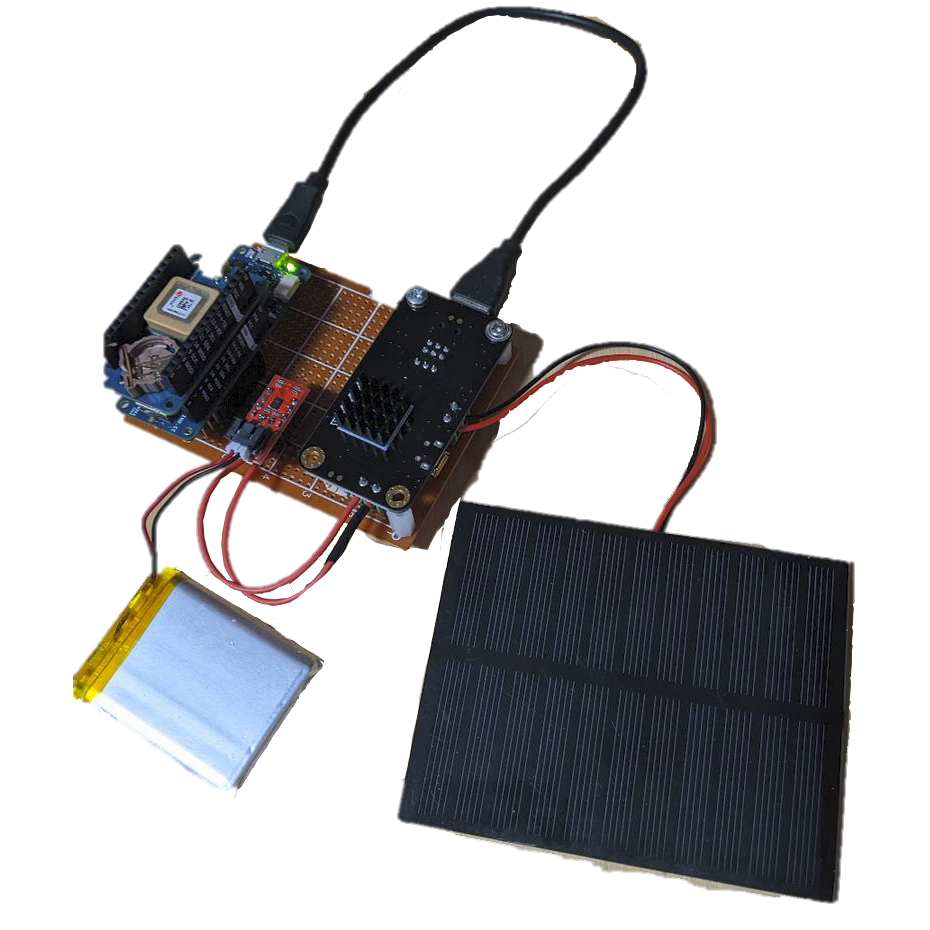
\includegraphics[width=0.5\textwidth]{./figs/prototype_clean.png}
  \caption{Prototype of the reinforcement learning-enabled cattle tracker. The device consists of a solar panel for power harvesting, a rechargeable battery, and an embedded microcontroller for decision-making and communication.}
  \label{fig:prototype}
\end{figure}

The system was evaluated based on its power consumption, data transmission efficiency, and overall performance in real-world conditions. The reinforcement learning algorithm optimized the power usage by balancing data collection, storage, and transmission to ensure continuous operation.

Additionally, the power levels of the device over time were analyzed to assess energy efficiency. Figure~\ref{fig:power_levels} shows the variation in power consumption during different operational phases.

\begin{figure}[htbp]
    \centering
    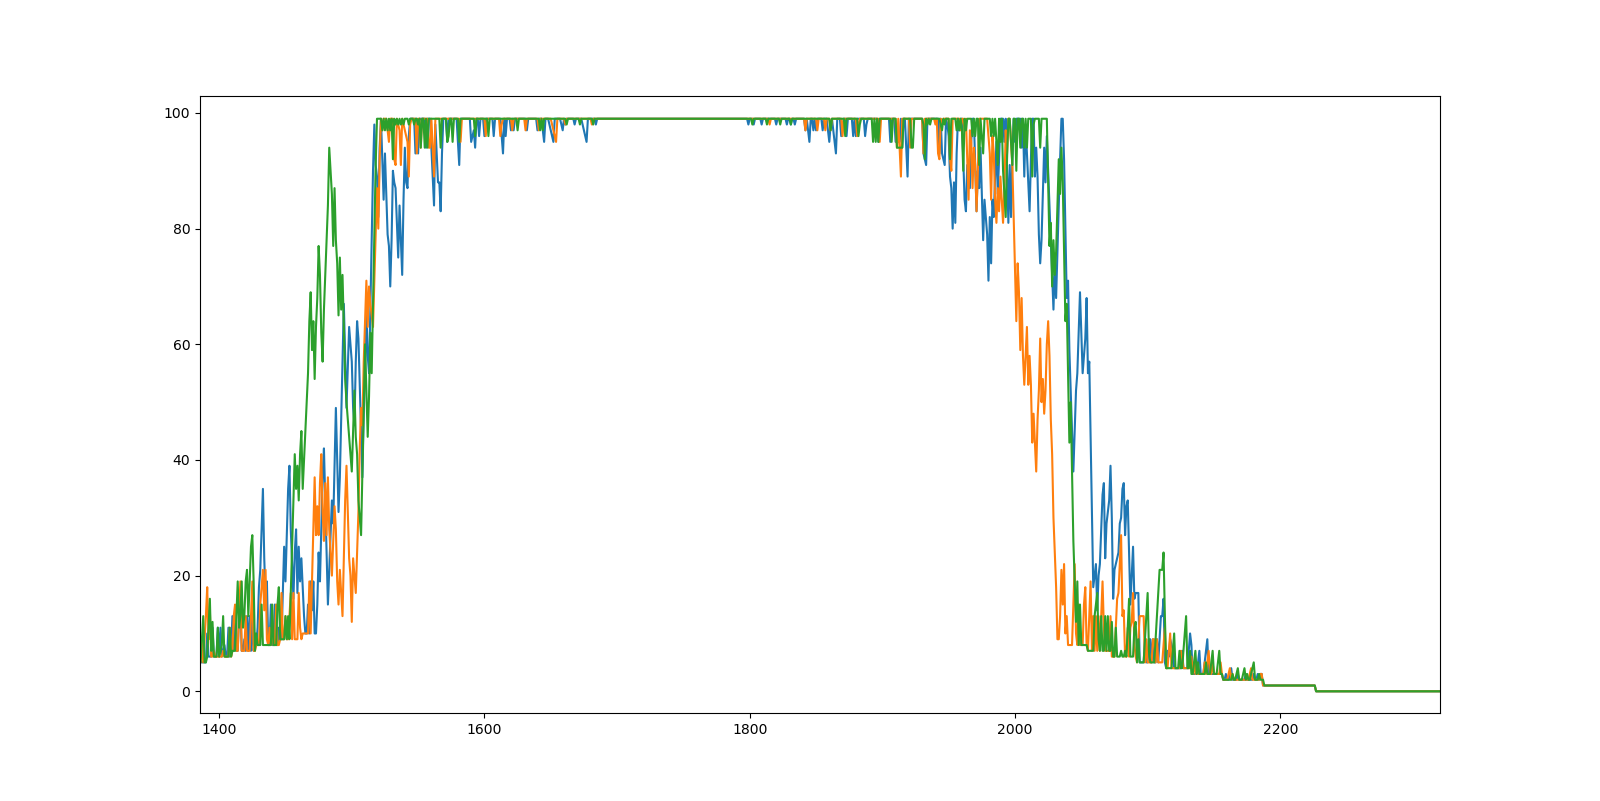
\includegraphics[width=0.8\textwidth]{./figs/power_levels.png}
    \caption{Power consumption levels of the cattle tracker over time. Different colors represent different operational phases such as data transmission, storage, and idle states.}
    \label{fig:power_levels}
\end{figure}


\section{Conclusion}


\section*{Acknowledgements}
We would like to acknowledege the funding provided by NeurAlbertaTech for this project.

%Appendixes go here
\appendix

\section{Example of math equation }
%\label{appendix-customize-this-label}
Binomial theorem: \cite{hribarUsingDeepQLearning2019}
\begin{equation}
(x+y)^n=\sum_{\substack{k=0}}^{n}\dbinom{n}{k}x^{n-k}y^k
\end{equation}


% All references should be stored in the file "references.bib".
% That call to use that file is in "cai.cls". 
% Please do not modify anything below this line.
\printbibliography[heading=subbibintoc]

\end{document}
